\documentclass[12pt]{article}   
\usepackage{geometry}
\geometry{letterpaper, margin=1in}
\parindent = 0pt

\usepackage{enumitem}
\usepackage{amssymb}
\usepackage{amsmath}
\usepackage[mathscr]{euscript}
\usepackage{extpfeil}
\usepackage {graphicx}
\usepackage{mathtools}
\usepackage{changepage}
\usepackage{tikz}
\usepackage{ulem}
\usepackage{float}
\usepackage{subcaption}

\usepackage{amsthm}
\newcommand{\RR}{\mathbb{R}}
\newcommand{\ZZ}{\mathbb{Z}}
\newcommand{\QQ}{\mathbb{Q}}
\newcommand{\NN}{\mathbb{N}}

\newcommand*\circled[1]{\tikz[baseline=(char.base)]{
            \node[shape=circle,draw,inner sep=2pt] (char) {#1};}}


\theoremstyle{definition}

\newtheorem*{defn}{Definition}
\newtheorem*{claim}{Claim}
\newtheorem{ex}{Example}

\begin{document}

\large
Counting Triangles \\
\normalsize

We asked the Math Circle students how many triangles are in the following pictures:

% Figure with two example triangle-counting problems
\begin{figure}[H]
	\centering

	% Subfigure with 2x2 triangle
	\begin{subfigure}{0.4 \textwidth}
		\centering
		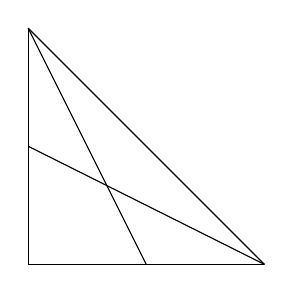
\begin{tikzpicture}[scale = 3]
		\draw (0, 1) -- (1, 0);
		\draw (0, 1) -- (0.5, 0);
		\draw (0, 1) -- (0, 0);
		\draw (1, 0) -- (0, 0.5);
		\draw (1, 0) -- (0, 0);
		\end{tikzpicture}
		\caption{There are 8 triangles here}
	\end{subfigure}
	%
	% Subfigure with 3x3 triangle
	\begin{subfigure}{0.4 \textwidth}
		\centering
		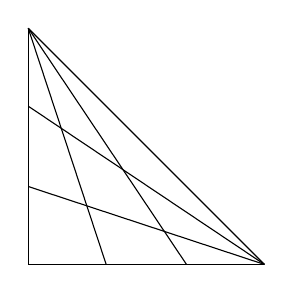
\begin{tikzpicture}[scale = 3]
		\draw (0, 1) -- (1, 0);
		\draw (0, 1) -- (0.67, 0);
		\draw (0, 1) -- (0.33, 0);
		\draw (0, 1) -- (0, 0);
		\draw (1, 0) -- (0, 0.67);
		\draw (1, 0) -- (0, 0.33);
		\draw (1, 0) -- (0, 0);
		\end{tikzpicture}
		\caption{There are 27 triangles here}
	\end{subfigure}
\end{figure}

We want to find a formula for the number of triangles in the more general picture:

% Figure with nxm triangle
\begin{figure}[H]
	\centering

	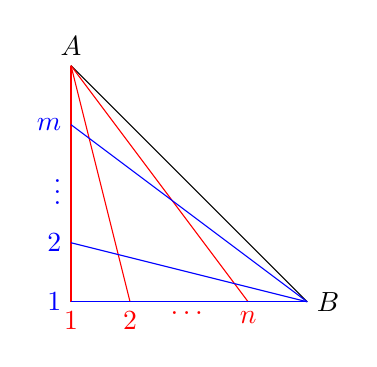
\begin{tikzpicture}[scale = 3]
	\draw (0, 1) node[above] (A) {$A$} -- (1, 0) node[right] (B) {$B$};
	\draw[red] (0, 1) -- (0.75, 0) node[below] (An) {$n$};
	\draw[red] (0.5, 0) node[below] (Adots) {$\dots$};
	\draw[red] (0, 1) -- (0.25, 0) node[below] (A2) {2};
	\draw[red] (0, 1) -- (0, 0) node[below] (A1) {1};
	\draw[blue] (1, 0) -- (0, 0.75) node[left] (Bm) {$m$};
	\draw[blue] (0, 0.5) node[left] (Bdots) {$\vdots$};
	\draw[blue] (1, 0) -- (0, 0.25) node[left] (B2) {2};
	\draw[blue] (1, 0) -- (0, 0) node[left] (B1) {1};
	\end{tikzpicture}

\end{figure}

To count the triangles in the general picture, notice that every triangle includes vertex $A$ or vertex $B$. By the Inclusion-Exclusion Principle, the total number of triangles is
$$\# A \text{ triangles } + \# B \text{ triangles} - \# AB \text{ triangles}.$$

\begin{claim} In the case where $m = n$, the number of triangles is $n^3$.
	\begin{proof} 
	Let $T_n$ be the $n$th triangular number, so
	$$T_n = \binom{n + 1}{2}.$$
		
	Counting with the Inclusion-Exclusion Principle, the number of triangles is
	\begin{multline*} n \cdot T_n + n \cdot T_n - n^2 = n \cdot (T_n + T_{n-1} + n) - n^2 
	= n \cdot (n^2 + n) - n^2 = n^3 + n^2 - n^2 = n^3 \end{multline*}
	
	Equivalently, we could use binomial coefficients and get
	$$ 2n \cdot \binom{n + 1}{2} - n^2 = \frac{2 n (n + 1)!}{2! (n - 1)!} - n^2
	= n^2 \cdot (n + 1) - n^2 = n^3 $$
	\end{proof}
\end{claim}

\newpage

\begin{claim} More generally, for $m, n \in \NN$ the number of triangles is $m \cdot n \cdot \frac{n + m}{2}$.
	\begin{proof} Again, let $T_n$ represent the $n$th triangular number, and let $T_m$ represent the $m$th triangular number. Counting as before, the number of triangles is
	\begin{multline*} m \cdot T_n + n \cdot T_m - m \cdot n = m \cdot \binom{n + 1}{2} + n \cdot \binom{m + 1}{2} - m \cdot n \\
	= \frac{m (n + 1)!}{2! (n - 1)!} + \frac{n (m + 1)!}{2! (m - 1)!} - m \cdot n = \frac{m \cdot n \cdot (n+1) + n \cdot m \cdot (m+1)}{2} - m \cdot n \\
	= \frac{m \cdot n^2 + n \cdot m^2}{2} = m \cdot n \cdot \frac{n+m}{2} \end{multline*}
	As expected, in the special case where $m = n$ we have
	$$m \cdot n \cdot \frac{n+m}{2} = n \cdot n \cdot \frac{n+n}{2} = n^3.$$
	\end{proof}
\end{claim}

Here are some examples of $n$ and $m$ values, and the total number of triangles they produce. Notice that the first row and column are the triangular numbers, and the main diagonal is the cubic numbers. \\

$$\bordermatrix{\text{$n, m$}	& 	1	&	2	&	3	&	4	&	5	&	6	&	7 \cr
                		1			&	1	&	3	&	6	&	10	&	15	&	21	&	28 \cr
                		2			& 	3	&	8	&	15	&	24	&	35	&	48	&	63 \cr
			3			&	6	&	15	&	27	&	42	&	60	&	81	&	105 \cr
			4			&	10	&	24	&	42	&	64	&	90	&	120	&	154 \cr
			5			&	15	&	35	&	60	&	90	&	125	&	165	&	210 \cr
			6			&	21	&	48	&	81	&	120	&	165	&	216	&	273 \cr
			7			&	28	&	63	&	105	&	154	&	210	&	273	&	343}$$


\end{document}


